En este capítulo se presentará el estado del arte en lo que respecta a los distintos usos de las bioseñales. Primero se mostrará el uso de las bioseñales en Accesibilidad, luego su uso en aplicaciones interactivas y finalmente se sacarán conclusiones. 

\section{Uso de bioseñales en distintos campos}

La computadora utilizada por Stephen Hawking es tal vez el caso más conocido de la utilización de bioseñales en Accesibilidad. Stephen Hawking cuenta con esclerosis lateral amiotrófica, por lo que se encuentra paralizado y no puede hablar. Para poder comunicarse, Intel desarrolló un sistema compuesto por una tableta y un sensor infrarojo montado en sobre sus anteojos. El sensor infrarojo detecta el movimiento en su cachete izquierdo. La tableta cuenta con una plataforma de código abierto llamada ACAT. ACAT provee un teclado virtual en la pantalla. Utilizando el movimiento de su cachete, Hawking, puede detener el cursor donde desea y así, escribir. Es decir, es una entrada binaria. Este también utiliza un procesador de texto con predicción de palabras que permite acelerar el proceso.  Luego, el sistema utiliza un sintetizador de voz para comunicar lo que escribió. Esta, es solo una de las aplicaciones de ACAT. ACAT también le permite controlar el ratón en \emph{Windows}, y así, controlar completamente la computadora para poder utilizar su correo electrónico, navegar por internet, entre otras cosas \cite{hawking}.

La NASA desarrolló un sistema para controlar un avión en una simulación utilizando los movimientos musculares medidos con sensores EMG(Electromiografía). Colocaron diversos sensores sobre una manga de tela. Con ellos, adquirieron la señal y la filtraron y eliminaron el ruido. Luego extrajeron las características y reconocieron patrones en una fase de entrenamiento. Con esta información, se aplicaron patrones de reconocimiento en una simulación interactiva. Lograron controlar un avión de guerra sin utilizar una palanca de mando. Es decir, el usuario colocaba la mano como si estuviese utilizando una palanca de mando y realizaba movimientos para controlar el avión (ver figura \ref{fig:emg-flight}) \cite{emg-flight}.

\begin{figure}[H]
	\centering
    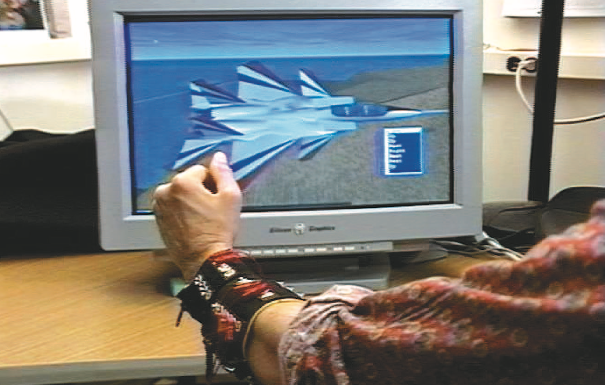
\includegraphics[width=0.8\textwidth]{emg-flight.png}
    \caption{Un usuario utilizando el dispotivo EMG para controlar un avión en una simulación.}
	\label{fig:emg-flight}
\end{figure}

Dos académicos de la Universidad Nacional de Seúl, utilizaron un dispositivo EMG y un acelerómetro para controlar un video juego. Utilizando el acelerómetro, el juego era capaz de determinar si el usuario estaba dando un simple puñetazo hacia adelante, un puñetazo de abajo hacia arriba o si estaba lanzando una bola de fuego (ver 
figura \ref{fig:fireball}). Usando el sensor EMG, el juego medía la fuerza realizada por el usuario y la aplicaba proporcionalmente en el juego. Es decir, si el usuario realizaba poca fuerza, el ataque era débil. En cambio, si era fuerte, el ataque era fuerte .De esta forma, se utilizó como dispositivo de entrada las propias señales del cuerpo en lugar de usar un control de mando físico o el teclado \cite{emg-fireball}.

\begin{figure}[H]
    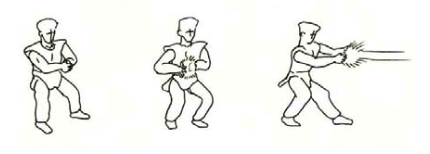
\includegraphics[width=0.8\textwidth]{emg-fireball.png}
    \caption{Movimiento realizado para lanzar una bola de fuego.}
	\label{fig:fireball}
\end{figure}

La empresa \emph{Muse} desarrolló un dispositivo EEG con cinco electrodos. El mismo viene acompañado con una aplicación móvil que ayuda a los usuarios a meditar. Cuando el usuario tiene la mente tranquila, se escucha un clima calmo, pero cuando el usuario está alterado se escucha un clima tormentoso. Muse utiliza distintas ondas cerebrales para detectar si el usuario se encuentra relajado o no.

\emph{Netflix} desarrolló \emph{MindFlix}. \emph{Mindflix} utiliza un dispositivo EEG (electroencefalograma) para controlar su popular servicio con la mente. Utiliza los giroscopios del dispositivo para permitirle al usuario desplazarse horizontalmente y verticalmente por la interfaz. Además, utiliza distintas ondas cerebrales para detectar cuando el usuario piensa en la palabra \emph{play}. En caso de que el usuario piense en esa palabra,  la aplicación comienza a reproducir el contenido seleccionado. Se intentó averiguar qué ondas cerebrales se utilizaban y de que forma no se encontró en ningun lugar \cite{mindflix}.


\section{Conclusiones}

Las aplicaciones de las bioseñales son infinitas y cada vez hay más interés en su uso. Pueden utilizarse tanto para ayudar a personas con discapacidad como también para entretener o para reemplazar sistemas físicos con virtuales. Todas las implementaciones combinan \emph{harware} y \emph{sowftware} pero algunas más que otras. En el caso de la computadora de Stephen Hawking, si bien utiliza un sensor infrarojo, el logro aquí está en el software que utiliza ya que el sensor no es tan sofisticado. En los casos de \emph{MindFlix} y \emph{Force Trainer}, el harware cobra más importancia, ya que las ondas del cerebro son difíciles de leer y se debe obtener el menor ruido posible. En el caso de controla un avión, el sensor es crucial pero a su vez lo es utilizar poderosos algoritmos para filtrar y limpiar las señales y para interpretar esas señales como distintos movimientos.

Sin duda han sido los avances tecnológicos de los últimos años los que han logrado que se haya podido avanzar tanto en esta área. Antes estos eran estudios realizados en laboratorios con equipamientos costos y específicos. En cambio hoy, existen diversos dispositivos accesibles para los consumidores. 